\notechapter{N-20241026}{Zariski Geometry: Varieties, Coordinate Rings, and Sheaves Without Fear}

\section{The algebra-geometry dictionary}

Affine algebraic geometry begins with polynomial equations. Given an ideal
\[
  I\subset k[x_1,\ldots,x_n],
\]
its zero set is
\[
  V(I)=\{a\in k^n:f(a)=0\text{ for all }f\in I\}.
\]
Conversely, for a set \(X\subset k^n\), the ideal of functions vanishing on it is
\[
  I(X)=\{f:f(x)=0\text{ for all }x\in X\}.
\]

\[
\begin{array}{c|c}
\text{geometry} & \text{algebra}\\
\hline
\text{affine variety} & \text{radical ideal}\\
\text{irreducible variety} & \text{prime ideal}\\
\text{regular functions} & \text{coordinate ring}\\
\text{local behavior} & \text{localization / stalks}
\end{array}
\]

\section{Coordinate rings}

If \(X=V(I)\), its coordinate ring is
\[
  k[X]=k[x_1,\ldots,x_n]/I(X).
\]
This is the ring of polynomial functions on \(X\).

Example: for the parabola \(X=V(y-x^2)\),
\[
  k[X]=k[x,y]/(y-x^2)\cong k[x].
\]
The parabola is algebraically the same as a line, even though it is drawn curved in the plane.

\section{Nullstellensatz as a promise}

Over an algebraically closed field, Hilbert's Nullstellensatz says that ideals and algebraic sets match after taking radicals:
\[
  I(V(I))=\sqrt I.
\]
This tells us that the algebra of polynomial equations remembers the geometry of their common zero set, up to nilpotent information.

\[
  \text{radical ideals are the algebraic shadows of affine varieties.}
\]

\section{The Zariski topology}

Closed sets in the Zariski topology are algebraic sets. This topology is much coarser than the usual Euclidean topology. For example, in \(\mathbb A^1\), proper closed sets are finite sets.

This feels strange at first. But the Zariski topology is designed so that polynomial functions behave naturally. It is not meant to measure physical closeness; it measures algebraic dependence.

\begin{figure}[H]
\centering
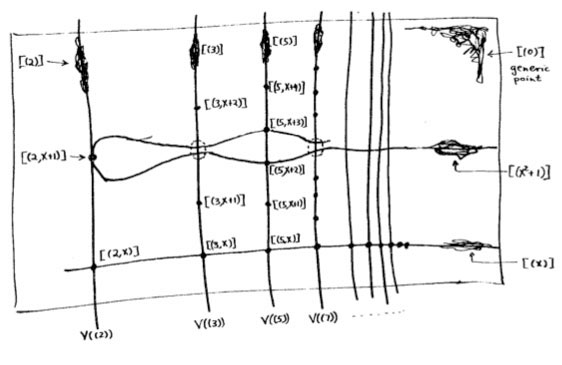
\includegraphics[width=.45\linewidth]{figures/N-20241026/mumforddrawing.jpg}
\caption{A useful mental picture: algebraic geometry keeps functions, equations, and shapes tied together.}
\end{figure}

\section{Regular functions are local}

On affine space, polynomial functions are regular. On more general open subsets, regular functions may look like fractions
\[
  \frac{f}{g},
\]
where \(g\) does not vanish on the open set being considered.

This locality is crucial. Geometry is not only about global polynomial formulas; it is about functions that are locally polynomial fractions.

\section{Why sheaves appear}

A sheaf is a device for keeping track of local data and gluing it when the local pieces agree. For regular functions, the sheaf condition says:
\[
\begin{array}{c}
  \text{if functions are defined locally,}\\
  \text{and they agree on overlaps,}\\
  \text{then they glue to a unique global function.}
\end{array}
\]
This is not abstract decoration. It is exactly what one expects of functions on a space.

\section{Stalks and germs}

The stalk of a sheaf at a point \(p\) stores the local behavior near \(p\). For regular functions, elements of the stalk are germs: two functions define the same germ if they agree on some neighborhood of \(p\).

The stalk is the algebraic microscope of the variety. It ignores what happens far away and keeps what can be seen arbitrarily close to the point.

%% expanded-on-review

\section{Distinguished opens by example}

In \(\mathbb A^1=\operatorname{Spec}k[x]\), the open set
\[
  D(x)=\{\text{points where }x\ne0\}
\]
corresponds to allowing \(x\) in denominators. The regular functions on this open set are Laurent polynomials
\[
  k[x,x^{-1}].
\]
This is the simplest example of localization.

In \(\mathbb A^2\), the open set \(D(x)\) removes the \(y\)-axis. On it, \(1/x\) is a perfectly regular function. This is why regular functions cannot be understood only as global polynomials on the whole ambient space.

\section{Sheaf gluing in a familiar case}

Cover a space by two open sets \(U\) and \(V\). Suppose we have a regular function \(f_U\) on \(U\) and a regular function \(f_V\) on \(V\). If
\[
  f_U|_{U\cap V}=f_V|_{U\cap V},
\]
then the sheaf condition says there is a unique function \(f\) on \(U\cup V\) restricting to both.

This may sound obvious for ordinary functions. That is precisely why it is the correct abstraction. Sheaves formalize the ordinary behavior of local data.

\section{A warning about pictures}

The Zariski topology is too coarse to be drawn faithfully. A line with the Zariski topology is not like a line with the Euclidean topology. Removing finitely many points still leaves a large open set.

So pictures in algebraic geometry should be treated as memory aids, not literal topology. The reliable object is the dictionary between equations, ideals, rings, and local functions.



\section{One more example: the hyperbola}

Let
\[
  X=V(xy-1)\subset\mathbb A^2.
\]
Its coordinate ring is
\[
  k[X]=k[x,y]/(xy-1).
\]
Since \(xy=1\), the element \(x\) is invertible and \(y=x^{-1}\). Hence
\[
  k[X]\cong k[x,x^{-1}].
\]
So the hyperbola is algebraically the affine line with the origin removed. This example is a good reminder that coordinate rings often reveal a simpler shape than the drawing suggests.


\section{What to remember}

Zariski geometry is not ordinary geometry with a weird topology. It is geometry rebuilt around polynomial functions.

\[
\begin{array}{c}
  \text{equations define spaces,}\\
  \text{functions on spaces form rings,}\\
  \text{local functions form sheaves,}\\
  \text{stalks record what happens near a point.}
\end{array}
\]
